~\vspace{.1in}

\section{Slopes}

Last week our supplier delivered 13 cases of paper for the office and charged us \$534.87.  This week, they delivered 20 cases of paper for \$814.80. We assume that their charge includes a fixed delivery fee and per case cost, so the dependence must be linear.  We would like to understand their pricing scheme better by writing the equation.

What to do?  We can name the variables and put the information we are given into a table.  That's a start.  The variables must be
\begin{center}
\begin{tabular} {l} 
$C=$ total charge (\$) $\sim$ dep \\ 
$N =$ number of cases delivered (cases) $\sim$ indep \\
\end{tabular}
\end{center}
and we know
\begin{center}
\begin{tabular} {|c| |c |c|}\hline
$N$ & 13 &  20\\ \hline
$C$ &534.87 & 814.80\\ \hline
\end{tabular}
\end{center}

Let's see.  The fixed delivery fee that we don't know is the intercept.  The per case cost that we also don't know is the slope.  To write the linear equation we need to know both.

The slope is just the rate of change, so we can figure out the slope just from the information in our table.
\begin{eqnarray*}
\text{slope} & = & \text{rate of change} = \frac{\text{change dep}}{\text{change indep}} = \frac{\$814.80-\$534.87}{20-13 \text{ cases}} \\
& = & \frac{\$279.93}{7 \text{ cases}} = 279.93 \div 7 = \$39.99 \text{ per case}\\
\end{eqnarray*}
\vspace{-.5in} %VSPACE

\noindent  or, all at once, as
 \begin{eqnarray*}
\text{slope} & = & \text{rate of change} = \frac{\text{change dep}}{\text{change indep}} = \frac{\$814.80-\$534.87}{20-13 \text{ cases}} \\
& = & (814.80-534.87)\div(20-13)= \$39.99 \text{ per case}\\
\end{eqnarray*}
\vspace{-.5in} %VSPACE

\noindent  
Either way, each case costs \$39.99 and the slope is \$39.99 per case.  

Now that we know the slope, we can find the intercept.   At \$39.99 per case we would expect 13 cases to cost $$13 \text{ cases } \ast \frac{\$39.99}{\text{case}} = 13 \times 39.99 = \$519.87$$
But the story tells us 13 cases cost \$534.87.  The difference $\$534.87 - \$519.87 = \$15$ must be the delivery fee which is the intercept.  Remember $$\text{intercept} = \text{dep} -\text{slope}\ast\text{indep}= 534.87 - 39.99\times 13= \$15$$

Why did we use 13 cases?  No good reason.  Look what happens if we use 20 cases at \$814.80 instead.
$$\text{intercept} = \text{dep} -\text{slope}\ast\text{indep}= 814.80 - 39.99\times 20= \$15$$
Yup.  Still \$15 delivery fee.

The equation is linear so it fits our template
$$\text{dep} = \text{start} + \text{slope} * \text{indep}$$
and now that we know the slope and intercept, we can put those in to get our equation.
$$C = 15 + 39.99N$$
Let's check.  When $N = 13$ we get $$C=15 + 39.99 \ast 13 = 15 + 39.99 \times \underline{13} = \$534.87 \quad \checkmark$$
and when $N=20$ we get $$C=15 + 39.99 \ast 20 = 15 + 39.99 \times \underline{20} = \$814.80 \quad \checkmark$$
You can also check that the graph goes through the original two points we were given.  The intercept is \$15, but because of the scale it shows up as barely above \$0 on our graph.
\begin{center}
\scalebox {.8} {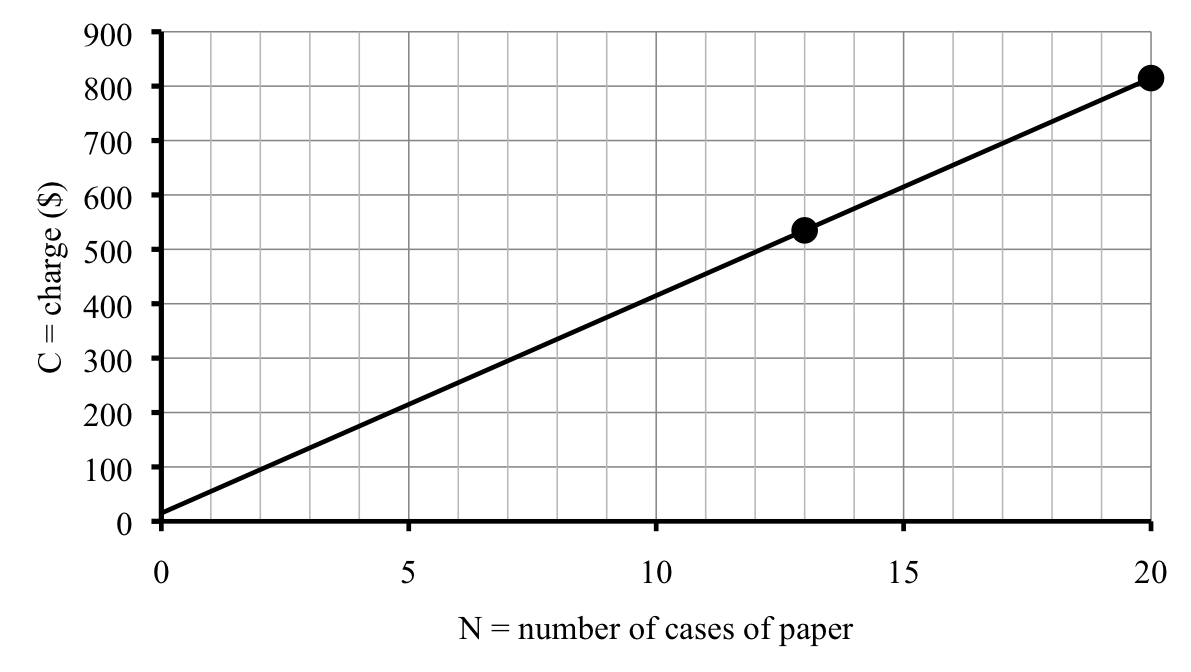
\includegraphics [width = 6in] {casesofpaper.png}}
\end{center}

The supplier also picks up recyclable paper and boxes.  The normally charge \$18 per pickup but under a new reuse incentive program, they discount a little for each box that's in good enough condition to use again.  This week's recycling charge was only \$7.60 because we returned the previous 13 boxes all in good shape.  

Now we're interested in how the recycling charge depends on the number of boxes in good condition that we return.  The new variables are
\begin{center}
\begin{tabular} {l} 
$R=$ recycling charge (\$) $\sim$ dep \\ 
$B =$ number of boxes returned (boxes) $\sim$ indep \\
\end{tabular}
\end{center}
and we know
\begin{center}
\begin{tabular} {|c| |c |c|}\hline
$B$ & 0 &  13\\ \hline
$R$ & 18 & 7.60\\ \hline
\end{tabular}
\end{center}
See how we used $B=0$ for the situation where no boxes are returned?  Clever.

We can draw the graph using just these two points.  (But we'll check later, once we have the equation, to be sure.) 
\begin{center}
\scalebox {.8} {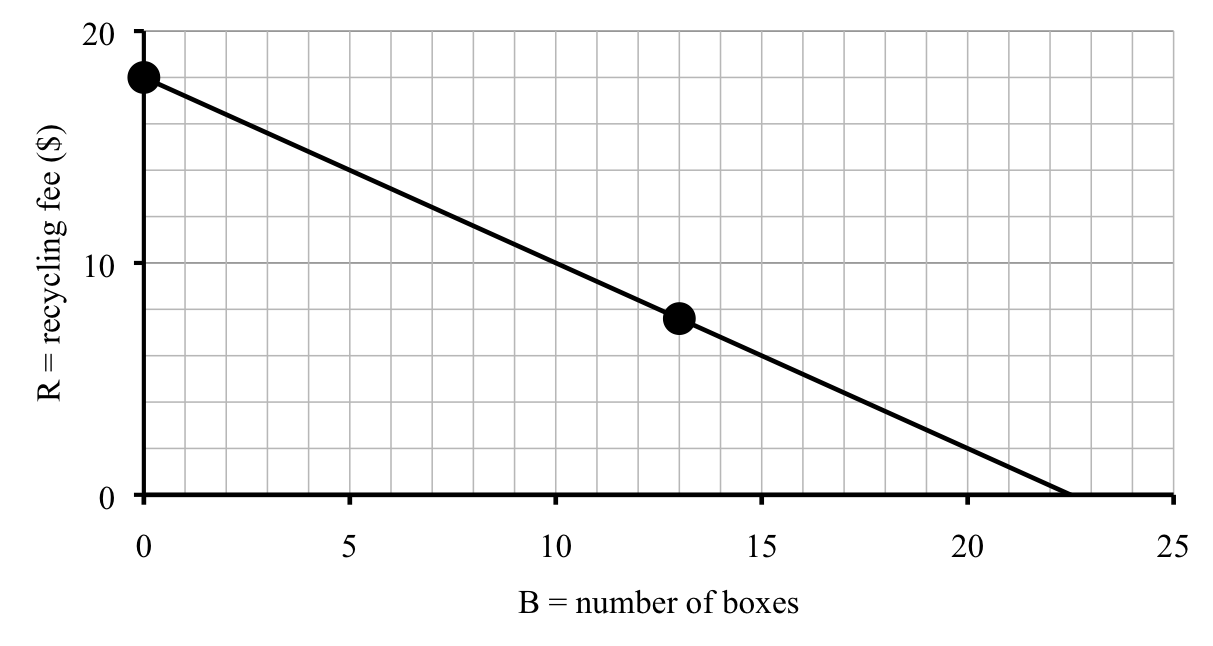
\includegraphics [width = 6in] {recyclepaper.png}}
\end{center}

Since there is a fixed discount per box, we again have a linear function.  We know the intercept is the normal recycling fee of \$18.  We need to find the slope.  
\begin{eqnarray*}
\text{slope} & = & \text{rate of change} = \frac{\text{change dep}}{\text{change indep}} = \frac{\$7.60-\$18}{13-0 \text{ cases}} \\
& = & (7.60-18)\div(13-0)= -\$.80 \text{ per box}\\
\end{eqnarray*}
\vspace{-.5in} %VSPACE

\noindent It might look funny to get a negative, but it's to be expected.  They are subtracting for each good box returned.  The discount is 80\textcent~per box and so the equation is
$$R = 18 - .8B$$
Check when $B=13$ we have $$R = 18 -.8*13 = 18-.8 \times \underline{13} = \$7.60 \quad \checkmark$$

What's the most boxes you could get credit for?  Probably the most they discount is the full \$18, which would mean that $R=0$.   That means we want to solve $ 18 -.8B = 0$. Check that we get $B = 22.5 \text{ boxes}$, which means that 22 boxes would be almost \$0 and for 23 boxes, they should pick up for free. We can check that 22 boxes gives $$R = 18-.8\ast22=18-.8 \times \underline{22} = \$.40$$
and 23 boxes gives
$$R = 18-.8\ast23=18-.8 \times \underline{23} = -\$.40 \implies \text{free}$$
Well, unless they're nice and give us cash back.

 %\section{Slopes}

\begin{center}
\line(1,0){300} %\line(1,0){250}
\end{center}

\section*{Homework}

\noindent \textbf{Start by doing Practice exercises \#1-4 in the workbook.}

\bigskip

\noindent \textbf{Do you know \ldots}

\begin{itemize} 
\item Which types of situations are linear? 
\item What the slope of a linear function means in the story and what it tells us about the graph? 
\item How to calculate the slope between two points? 
\item What is means if the slope is negative? 
\item How to find the equation of a line through two points? 
\item How to find a linear function given two examples in a story? 
\item If both the slope and intercept are unknown, which is easier to calculate first? 
\item[~] \textbf{If you're not sure, work the rest of exercises and then return to these questions.  Or, ask your instructor or a classmate for help.}
\end{itemize}

\subsection*{Exercises}

\begin{enumerate} 
\setcounter{enumi}{4}

\item  I just saw an advertisement for the same paper we use at the office for only  \$4.25 per ream at a supply store.  (Ream?  Yes.  That's 500 sheets of paper, usually wrapped in paper.) Is that a good deal?
\begin{enumerate}
\item There are 10 reams in a case.  What is the advertised price come to per case?
\item I'm not sure I want to go get a case of paper myself because a case of paper is pretty heavy to lift.  Paper is sold by the weight.  Thick, heavier paper is considered fancier than lighter paper.  The office uses a multipurpose paper called ``92'' meaning it weighs 92 grams per square meter which comes out to around 5 grams per sheet.  How much does a case weigh? Use $1 \text{ kilogram} \approx 2.2 \text{ pounds}$. % Go grams/sheet, sheet/ream, ream/case.
\item But, at the office we pay a delivery charge.  Compare the cost of having just one case delivered versus my buying one case at the store.  Recall that the office pays \$15 delivery fee and \$39.99 per case.
\item Write new equation for paper cost assuming I pick it up at the store. Use $N$ for the number of cases of paper and $C$ is the total cost, in dollars.
 \emph{Hint: this equation is a direct proportionality.}
\item Compare total cost if get 4 cases either delivered or from store.  Repeat 13 cases.  Recall that the equation for delivered paper is $C=15+39.99N$.
\item Graph both functions together on the same axes.
\item Set up and solve inequality for when delivered is cheaper.  
\end{enumerate}

\item The amount of garbage generated in the United States has increased steadily, from 88.1 million tons in 1960 to 254.2 million tons in 2006.  

\hfill \begin{footnotesize}  Source:  Environmental Protection Agency \end{footnotesize}
%  Link to data: http://www.epa.gov/osw/nonhaz/municipal/msw99.htm  Go to http://www.epa.gov/osw/nonhaz/municipal/pubs/msw_2010_rev_factsheet.pdf  for results, and data tables follow.  Added a bit about guess for 2010.

\hfill \emph{Story also appears in 4.5 Exercises}
\begin{enumerate}
\item Assume the amount of garbage increases linearly, by how much has garbage increased each year? 
\item Name the variables, including units, and write a linear equation relating them.
\item According to your equation, how much garbage was projected for 2010?  For 2020?
\item If this trend continues, when will the amount of garbage generated exceed 300 million tons?   Show how to set up and solve an inequality to find the answer.  Be sure to state the actual year.
\item A 2010 report listed the amount of garbage at 249 million tons.  Compare this information to your previous answer.  What are some possible explanations for why this amount was less than expected (and actually decreased from 2006)?
\end{enumerate} 

\item Now that he is retired, Elmer gets a pension check from the Railroad Company each month.  There's a set amount he gets each month but the company deducts a fixed percentage of whatever outside income he earns.  Elmer works part-time at the local hardware store.  In February he earned \$444.10 at the hardware store and his pension check that month was \$886.23.  In March he worked much less,  earning only \$179.30 at the hardware store; his pension check that month was \$912.71
\begin{enumerate}
\item What percentage of his income from the hardware store is deducted from his pension check?  \emph{Calculate the fraction of a dollar deducted for each dollar earned.  Convert your answer to percent.}
\item If Elmer doesn't work in April, how much will his pension check be?  
\item Write an equation showing how Elmer's pension check is affected by his income from the hardware store.  Use $H$ for his income from the hardware store and $P$ for his pension check, both in dollars.  
\item Elmer would like to earn enough at the hardware store to make at least \$1,200 total per month.  Using $T$ for the total Elmer earns in a month (in dollars), write an equation for $T$ as a function of $H$.  \emph{Hint:  start with $T=H+P$, then use your equation for $P$ from part (c) to write everything with $H$ instead.}
\item Now set up and solve an inequality to determine how much Elmer needs to earn at the hardware store to make at least \$1,200 total per month.
\item If Elmer earns \$8.15 per hour, how many hours does he need to work at the hardware store to make at least  \$1,200 total per month, accounting for his income from the hardware store and his pension check?
\end{enumerate}
 
\item Your local truck rental agency lists what it costs to rent a truck (for one day) based on the number of miles you drive the truck.  They use a linear pricing model.
\begin{center}
\begin{tabular} {|c| |c |c|c|c|} \hline
distance driven (miles) & 50 & 100 & 150 & 200 \\ \hline
rental cost (\$) & 37.50 & 55.00 & 72.50 & 90.00 \\ \hline
\end{tabular}
\end{center}
If you rent a truck and drive it 10 miles, how much do you think it will cost?  As part of your work, name the variables and write a linear equation relating them.

\hfill \emph{Story also appears in 1.2 and 1.3 Exercises}

\item In 2008, the median household income was about \$50,303.  By 2010 it was down to about \$49,445.
\hfill \begin{footnotesize} Source:  U.S. Census Bureau \end{footnotesize}
 % source:  http://www.census.gov/hhes/www/income/data/statemedian/index.html  Access Excel spreadsheet Median Household Income by State - Single-Year Estimates
\begin{enumerate}
\item By how much has it decreased each year, on average? The phrase ``on average'' means that you should assume the decrease is linear.
\item Name the variables and write a linear equation relating them.
\item At this rate when will the median family fall below \$48,000?  Set up and solve an inequality.
\item Graph and check.
\end{enumerate}

\item Buoy instruments in the oceans report changes in the sea level.  In 2005 the sea level (averaged across all the oceans) was 51.7 millimeters above the historical sea level.  In 2012 the sea level was 73.4 millimeters above the historical sea level.  You can assume the increase is linear.
\hfill \begin{footnotesize} Source:  National Aeronautics and Space Administration \end{footnotesize}
\begin{enumerate}
\item Name the variables, including units.
\item Display the information from the story in a table.
\item What is the rate of increase for the sea level?
\item Write an equation relating the variables.
\item In what year will the sea level be 80 millimeters above the historical level?
\end{enumerate} % Assumes an annual growth of 3.1 mm /yr  Source: http://sealevel.colorado.edu/  Cut:  to NASA.

\end{enumerate}